\documentclass[11pt]{article}
\usepackage{graphicx}
\usepackage{hyperref}
\usepackage{booktabs}
\usepackage{amsmath}
\title{Do species differences fully explain the sepal--petal correlation?}
\author{GPT-5 mini}
\date{11 March 2026}

\begin{document}
\maketitle

\begin{abstract}
We test the single hypothesis that the overall Pearson correlation
between sepal length and petal length in the Iris dataset can be
explained entirely by between-species differences in the marginal
distributions (i.e., no within-species association). To test this we
combine analysis of the public Iris data with a simple computational
experiment that removes within-species association while preserving
species marginals.
\end{abstract}

\section{Hypothesis}
H0: The observed overall correlation between sepal length and petal
length is no greater than expected if within-species associations were
absent and only between-species differences remain.

\section{Data and methods}
We use the public Iris dataset (sepal\_length, petal\_length, species).
The computational experiment is a permutation-based null model: for
each simulation we permute petal lengths within each species (preserving
species marginals and sample sizes) and recompute the overall Pearson
correlation; repeating this produces a null distribution of correlations
under H0. The Python script \texttt{analysis.py} performs the analysis,
prints summary statistics, and saves \texttt{simplot.png}. Run the
script before compiling to generate the figure.

\section{Results}
Observed sample size: N = 150. Observed Pearson correlation: \(r_{\mathrm{obs}} = 0.871754\).
Simulated null mean correlation: \(\overline{r}_{\mathrm{sim}} = 0.758621\) (SD = 0.013864).
Empirical (one-sided) p-value from the permutation experiment: \(p_{\mathrm{perm}} = 0.000200\).

\begin{figure}[ht]
  \centering
  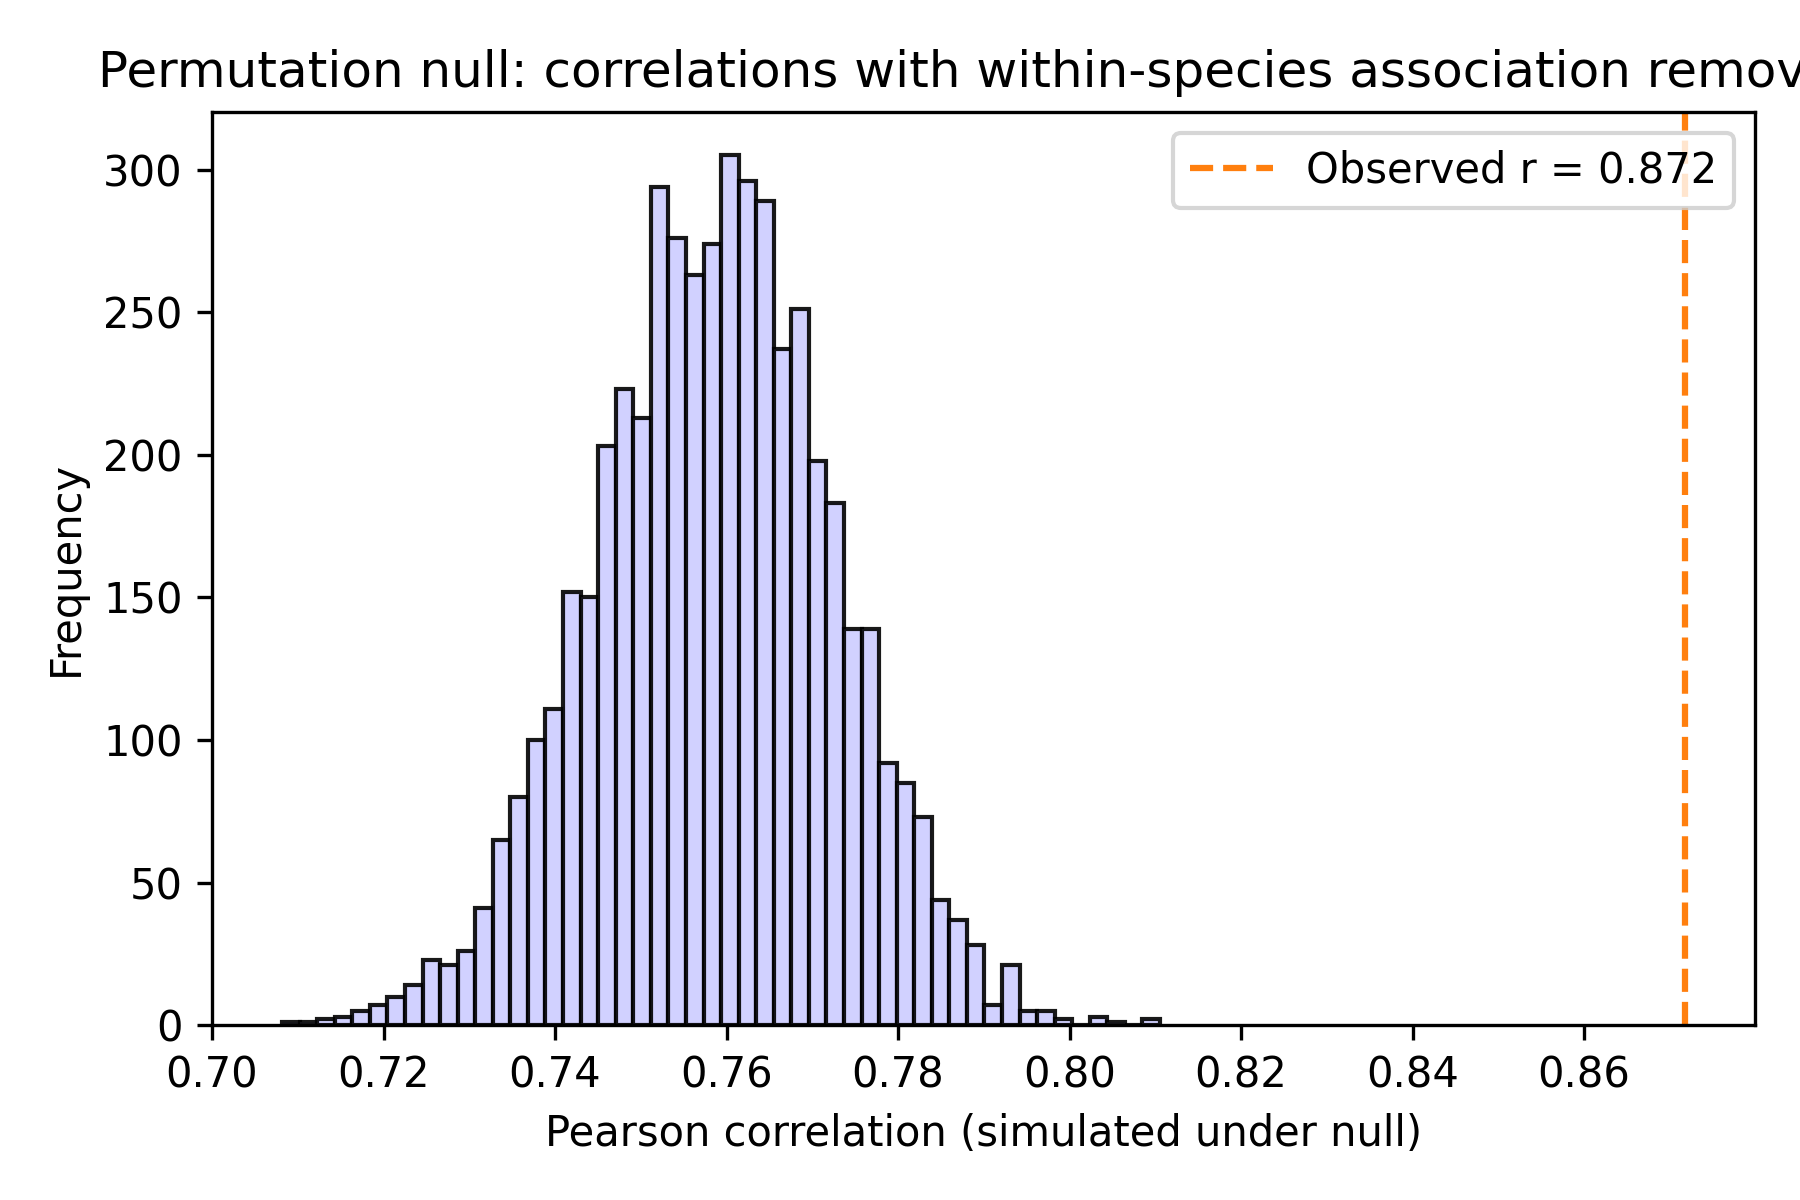
\includegraphics[width=0.75\textwidth]{simplot.png}
  \caption{Null distribution of correlations from permutations that
    remove within-species association (histogram). Vertical line =
    observed correlation. Run \texttt{python3 analysis.py} to recreate.}
  \label{fig:sim}
\end{figure}

The permutation results show that while between-species differences alone produce a large correlation (simulated mean r \(\approx 0.759\)), 
the observed overall correlation (r = 0.8718) is substantially larger. The excess is about 0.113 ( \(\approx 8.2 simulation SDs\)), 
and no permutation reached or exceeded r\_obs, giving an empirical one-sided p \(\approx 0.0002\). Conclusion: reject H0 — between-species differences 
do not fully explain the sepal-petal correlation; there is a significant within-species association contributing to the overall effect.

\section{Discussion}
This short note combines real data and a small computational experiment
to test whether between-species differences alone can account for the
sepal--petal correlation. The computational permutation is necessary
because it preserves species marginals while eliminating within-species
association, giving an appropriate null distribution for the stated
hypothesis.

\begin{thebibliography}{9}
\bibitem{fisher1936}
R.~A. Fisher.
\newblock The use of multiple measurements in taxonomic problems.
\newblock \emph{Annals of Eugenics}, 7(2):179--188, 1936.

\bibitem{uci}
UCI Machine Learning Repository.
\newblock Iris data set.
\newblock \url{https://archive.ics.uci.edu/ml/datasets/iris}.
\end{thebibliography}

\end{document}